\chapter{Black Holes and Active Galactic Nuclei}
In this chapter we will explore a topic that stands between cosmology and small scale astrophysics: with the technological improvements that lead to the building of the first radio telescopes, astronomers found themselves puzzled by the discovery of curious objects that appear to be stars, but behave very differently from regular stars. The search for a physical model that could describe these quasi stellar (which today we call QuaSaRS, or Quasi Stellar Radio Sources) sources lead a deep investigation of black hole physics; moreover, the fact that these mysterious objects could reach a mass as high as $10^9 M_\odot$ raised the questions on how such massive astrophysical bodies could be even put together in the period of time that elapses from recombination to the highest QUASAR observed redshift $z_{QSRS}\approx7$. We will explore these questions, and some possible answers, in this chapter. 

\section{Motivation: a strange emission spectrum}
We already know, from chapter 7, that there is a variety of systems in our universe that behave as black bodies, with various temperatures $T$: the reason why is that basically every physical system that is in thermal equilibrium will emit electromagnetic radiation which as a spectral distribution
\begin{equation}
B_\nu(T) = \frac{2h\nu^3}{c^2}\frac{1}{e^{h\nu/k_BT}-1}
\end{equation} 
where $T$ is the equilibrium temperature and $B_\nu$ is the amount of energy emitted in a certain frequency band $[\nu,\nu+d\nu]$, per unit area,time and direction (spectral radiance). A typical star, the sun, behaves as a black body with an equilibrium temperature of $T_\odot\approx 6000$\,K and emits a total luminosity
\begin{equation}
L_\odot = 4\pi R_\odot^2\int_{0}^\infty d\nu B_\nu(T_\odot)\approx 3.84\cdot 10^{33}\mathrm{erg}\,\mathrm{s}^{-1}
\end{equation}
You can imagine the look on the face of the guy that, during an observation session, detected with his radio telescope an object that was as small as a point (like a star), but had an output luminosity $L_{obj}\approx 10^{47}\mathrm{erg}\,\mathrm{s}^{-1}$, almost $10^{14}$ times bigger than the luninosity of the sun! There is no stellar physical model nowadays that can explain such a big energy output from a regular star. If that object were a star, it had to have a mass several billion times bigger than the sun, but this is impossible due to hydrodynamical instabilities that prevent stars so massive to even exist. Moreover, the spectral radiance that the same guy measured didn't resemble the one of a black body at all (just have a look at Figures \ref{quasarspecideal} and \ref{quasarspecreal})

\begin{figure}
\begin{center}
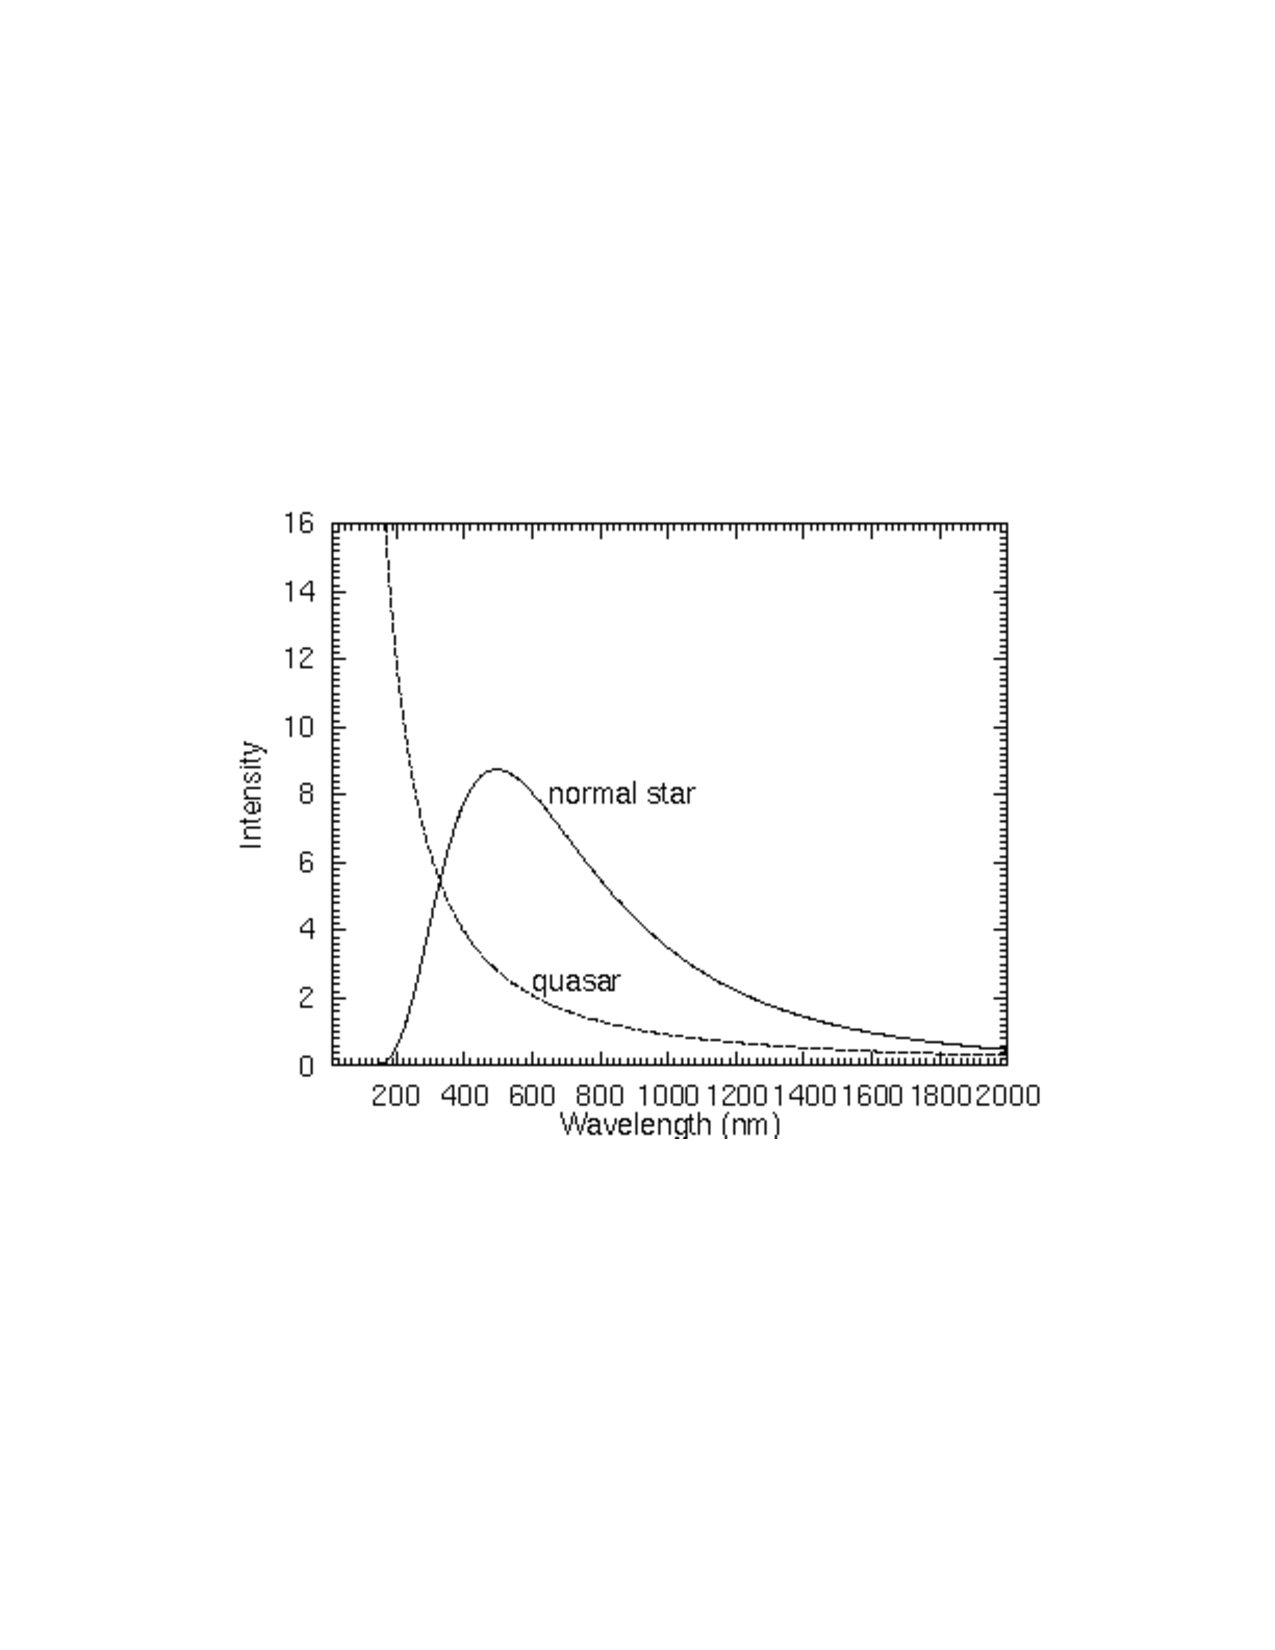
\includegraphics[scale=0.8]{Draw/quasar_spec_ideal.pdf}
\end{center}
\caption{Emission spectrum of Quasi Stellar Radio Sources compared to the one emitted by a regular star, credit for the image \url{http://www.astronomynotes.com/galaxy/plsync.gif}}
\label{quasarspecideal}
\end{figure} 

\begin{figure}
\begin{center}
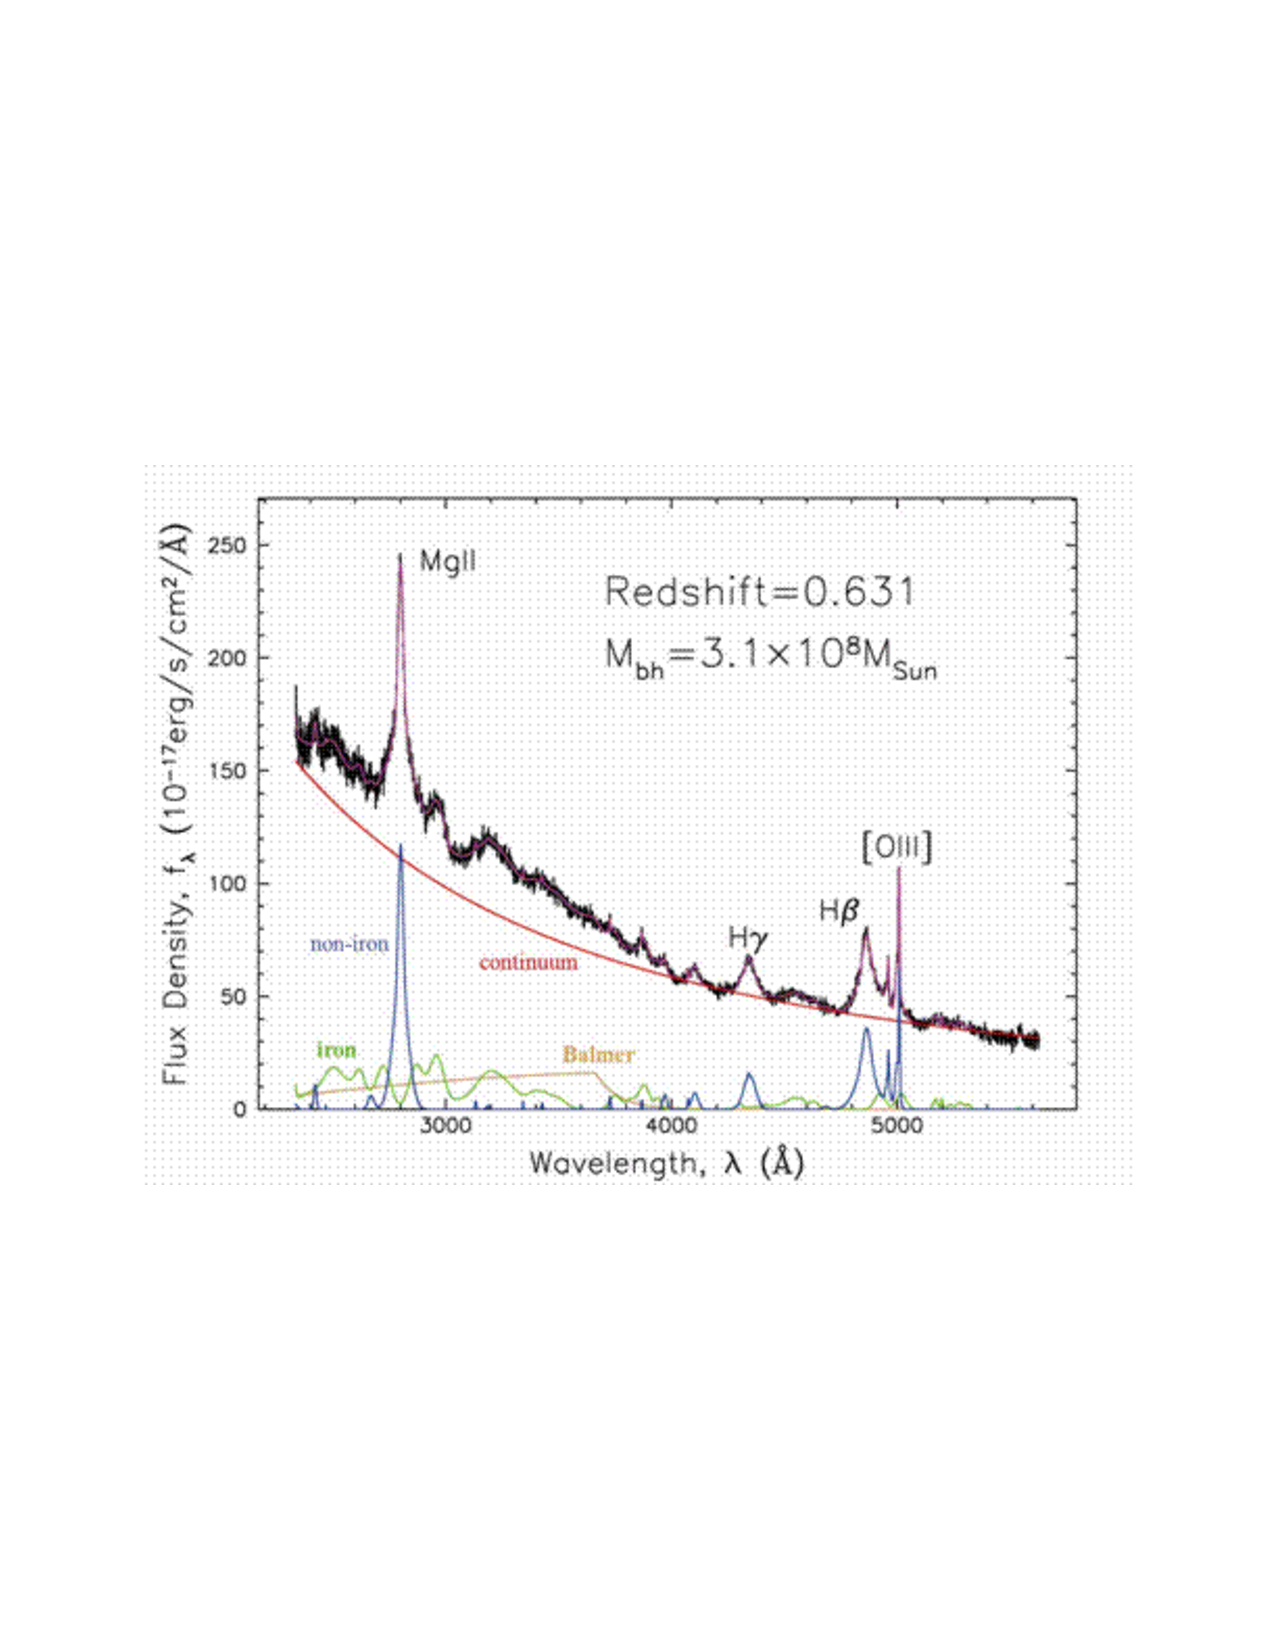
\includegraphics[scale=0.8]{Draw/quasar_spec_real.pdf}
\end{center}
\caption{Actual measurement of a QUASAR spectrum (bottom panel), credit for the image \url{http://grist.caltech.edu/images/fig1_annrep04.gif}}
\label{quasarspecreal}
\end{figure}  

\noindent Whatever mechanism lies behind such a strange emission spectrum and such a high luminosity, it cannot be a stellar one, for the reasons we stated above. What are these objects then? The answer might seem absurd, but the most widely accepted picture, as of today, is that these object are in reality heavy black holes that accrete the surrounding gas at a very high rate. These objects are also very far from us, the farthest one known to be approximately 9 billion light years away. In the following section we will explore the physics of these exotic objcets in more detail. 

\section{Black hole physics}
In this section we will try to understand better what a black hole is and, more important of all how can a system like this, once put in an appropriate environment, can emit such a huge amount of energy. 
\subsection{Isolated black holes}
Recall all the things about General Relativity we learned in Chapters 3 and 4; in particular recall how we measure the space time interval
\begin{equation}
ds^2 = g_{\mu\nu}dx^\mu dx^\nu
\end{equation}
The metric $g_{\mu\nu}$ is a solution of the Einstein's equation
\begin{equation}
G^{\mu\nu}=\frac{8\pi G}{c^4}T^{\mu\nu}
\end{equation}
where $G^{\mu\nu}$ is the Einstein tensor (that can be expressed in terms of the metric and its derivatives) and $T^{\mu\nu}$ is some tensor that describes the energy distribution in our spacetime. If the surrounding of our black hole is pure vacuum then $T^{\mu\nu}=0$ and Einstein's equation reduces to $G^{\mu\nu}=0$. This equation can be solved exactly if we assume that our black hole has a mass $M$ and is spherically symmetrical (i.e. is non rotating), and the solution is the famous Schwarzschild metric that, expressed in spherical coordinates looks something like
\begin{equation}
ds^2=-\left(1-\frac{2GM}{rc^2}\right)c^2dt^2 + \frac{dr^2}{1-\frac{2GM}{rc^2}} + r^2(d\theta^2+\sin^2\theta d\phi^2)
\end{equation}
Now we'll try to explore some of the physical properties of a metric in this form; first of all you may notice that something weird happens when $r=r_s\equiv 2GM/c^2$ (recall that for the sun $r_s\sim 2$km and for Earth $r_s\sim$ few cm). In particular we see that, as we cross the spherical surface $r=r_s$ from the outside to the inside $g_{00}$ vanishes and changes sign: this is what is called and \textit{event horizon}. Inside the horizon time and space swap roles (whatever this means, physics in the region $r<r_s$ is still very poorly understood); moreover inside the horizon, there is \textit{no spacetime trajectory} that has $dr=0$ (recall that spacetime trajectories always have $ds^2<0$). This means that no matter how hard one tries, there is no way that you can sit still inside a black hole horizon, you will always fall towards the center and hit the singularity, even if you sit on a spaceship whose engines are infinitely powerful. Let's examine another curious feature black holes exibit, and for which common sense intuition fails; suppose an observer finds itself sitting still at a distance of several $r_s$ away from the event horizon. This observer will start falling towards the singularity at a rate $\dot{r}=f(r)$ with $f(r)$ some function of the distance, that can be explicitely calculated in Newtonian mechanics or General Relativity (the two answers will be different of course). Suppose another observer sits at a safe distance, and looks at the first one falling inside the singularity. Let $t$ be the time measured by this safe standing observer. According to Newtonian mechanics the position $r(t)$ of the falling observer will change according to 
\begin{equation}
\frac{dr(t)}{dt}=-\sqrt{\frac{2GM}{r(t)}}=-c\sqrt{\frac{r_s}{r(t)}}
\end{equation}
We already know that when we take into account General Relativity the typical corrections that arise are of order $r_s/r$ and in fact the correct calculation of the infalling speed will give
\begin{equation}
\frac{dr(t)}{dt}=-\sqrt{\frac{2GM}{r(t)}}=-c\sqrt{\frac{r_s}{r(t)}}\left(1-\frac{r_s}{r}\right)
\end{equation}
One first surprising fact that we can immediately be aware of is that as $r\rightarrow r_s$, the infalling speed tends to 0; in fact the observer \textit{slows down} as it approaches the event horizon! This effect is purely general relativistic. And this is not all, if we try to actually compute the time $t_s$ that the observer takes to reach the event horizon
\begin{equation}
t_s = \int_{r_s}^{r_{initial}}\frac{dr}{dr/dt} = \frac{1}{c\sqrt{r_s}}\int_{r_s}^{r_{initial}}\frac{dr\sqrt{r}}{1-\frac{r_s}{r}}\propto -\log\left(\frac{r}{r_s}-1\right)_{r\rightarrow r_s}
\end{equation}
we quickly find that this time is infinite: the falling observer, as seen from outside, will never reach the event horizon! You will be surprised to learn that this statement is not true anymore in the free falling observer's reference frame. In this frame, the proper time interval that the observer measures is $ds = dt\frac{ds}{dt} = \left(1-\frac{r_s}{r}\right)dt$; this means that the falling observer's watch, will measure a time
\begin{equation}
t^{falling}_s = \int_{r_s}^{r_{initial}}\frac{dr}{dr/ds} = \frac{1}{c\sqrt{r_s}}\int_{r_s}^{r_{initial}}dr\sqrt{r}\propto \frac{r_{initial}^{3/2}}{c\sqrt{r_s}}
\end{equation}
between the start of the fall and the horizon crossing time. Note that this time is finite! In other words, the falling observer will fall into the black hole in a finite time, but in an external, inertial reference frame, an infinite amount of time will elapse. That's why a black hole can be seen as a very efficient time machine (that can only allow time travel in the future though...)
\subsection{Rotating black holes}
The spherical Schwarschild geometry is not the only solution to the Einstein equation in vacuum $G^{\mu\nu}=0$; relaxing the assumption of spherical symmetry Kerr found an exact solution to this equation that has only cylindrical symmetry (the same symmetry that for example describes a spherical spinning top). This solution is believed to describe spherical black holes that rotate along an axis $\hat{\mathbf{n}}$. The metric tensor $g_{\mu\nu}$ that describes this solution can be written in terms of the mass of the black hole $M$, its rotational angular velocity $\omega$ and the direction of the rotation axis $\hat{\mathbf{n}}$, but the expression is really long and complicated and cannot be contained in this page. What can be done in this page is describe qualitatively the spacetime geometry that this solution describes, which looks like Figure \ref{kerrBH}. The inner spherical surface has a radius 
\begin{equation}
r_H = r_s\frac{1+\sqrt{1-4\frac{\omega^2r_s^2}{c^2}}}{2}  
\end{equation}
where $r_s=2GM/c^2$. This surface at $r=r_H$ is an actual event horizon, and whatever falls in is destined to fall in the singularity. The outer surface, which we drew with a dashed line, is something peculiar of rotating black holes; Kerr gave it the name \textit{ergoshpere}. It has a $\theta$ dependent radius
\begin{equation}
r_{E}(\theta) =  r_s\frac{1+\sqrt{1-4\frac{\omega^2r_s^2}{c^2}\cos^2\theta}}{2}
\end{equation}
It is important in the sense that whatever observer is trapped between the ergoshpere at $r_E$ and the event horizon at $r_H$ has still a chance of not falling inside the singularity; it is still true though that an observer within the ergospher cannot stand still, but because the spacetime itself is spinning so fast, is forced to maintain a non zero orbital speed. This is why, even if the observer travels radially towards the center, once it crosses the ergosphere it will start rotating along with the black hole. This is another effect that is purely general relativistic. Should this observer escape from the ergosphere, it will draw some of the black hole spinning energy with him: this is what is called a \textit{Penrose process}, and it is one of the candidate models to explain the high energy gamma ray burst that are often captured by telescopes.   
\begin{figure}
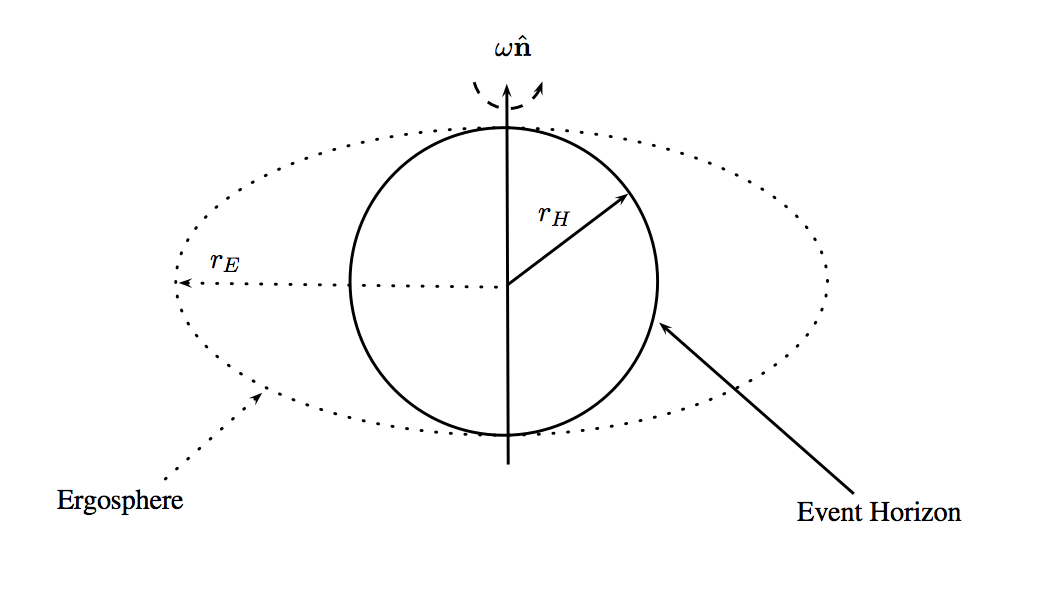
\includegraphics{Draw/kerrBH.png}
\caption{Geometrical picture of a rotating black hole}
\label{kerrBH}
\end{figure} 

\subsection{Black holes with surrounding gas clouds}  
So far we have explored the main physical features of isolated black holes: the main thing you should have noticed is that a black hole has an event horizon surrounding it, and this is the main reason why we gave it the adjective "black": whatever falls in this event horizon cannot escape, not even light. How can then black holes be candidates to explain the enormous luminosities emitted by QuaSaRS? The answer is that, in a more realistic scenarios, black holes are not isolated, but are surrounded by gigantic gas clouds. The enormous gravitational pull these black holes exert on the surrounding gas particles forces these to fall into the gravitational well, and to radiate their potential energy away. Let's try to be more quantitative: hydrodynamical simulations showed that typically the radiation emission happens at a distance $\sim 5r_s$ from the center, that's we will try to model this emission with Newtonian gravity (which at these distances will be accurate to $\sim 20\%$). Suppose the gas cloud is entirely made by atomic hydrogen (which if you recall is a bound state of an electron and a proton), and suppose the black hole has a mass $M$; on average a hydrogen atom that makes up the cloud will be pulled towards the center by a gravitational force
\begin{equation}
\mathbf{F}_g = -\frac{GMm_H}{r^2}\hat{\mathbf{r}}
\end{equation}
Where $m_H$ is the mass of a hydrogen atom. Falling towards the center, it will collide with other hydrogen atoms and radiate its gravitational potential energy away; call $L$ the total luminosity emitted by this system. This outgoing radiation will have a feedback effect on the infall, slowing it down: what is the maximum luminosity that this system can sustain without stopping the accretion process? The generated photons will interact with the bound electrons (with a typical cross section $\sigma_T=\frac{8\pi}{3}\left(\frac{e^2}{m_ec^2}\right)^2$ as we have seen in Chapter 7) and push them outwards. Each photon of energy $E$ will transfer a momentum $p=E/c$ to a particular electron; the photons combined action results in an outgoing force
\begin{equation}
\mathbf{F}_{rad}=\frac{L\sigma_T}{4\pi r^2 c}\hat{\mathbf{r}}
\end{equation}
Clearly if we want the accretion to continue we must have $(\mathbf{F}_g+\mathbf{F}_{rad})\cdot \hat{\mathbf{r}}\leq0$, which gives us an upper limit to the luminosity that our combined (black hole + cloud) system can radiate
\begin{equation}
L\leq L_{Edd} = \frac{4\pi c M_H G M}{\sigma_T}
\end{equation}
Where the subscript "Edd" stays for Eddington, as the name of the astronomer who first proposed this limit; let's put a few numbers here. First, what is the order of magnitude of this limit luminosity for a $1M_\odot$ black hole? We can calculate it straightforwardly:
\begin{equation}
L_{Edd}(1M_\odot)=\frac{4\pi c m_H G M_\odot}{\sigma_T}\approx 3.2\cdot 10^4 L_\odot
\end{equation} 
so we already see that a mechanism like this can output a luminosity bigger that $10^4$ the luminosity of the sun, even for a 1 solar mass black hole. Black holes are more efficient than nuclear reactors in producing energy! (provided you fuel them enough obviously). This Eddington luminosity scales linearly with the mass of the system, so you can see that a heavy black hole (of say $10^9M_\odot$) can easily reach the output luminosities we were talking about in the introduction to this chapter. If the gravitational pull of the black hole is big enough, the combined system can easily saturate this luminosity limit. When this happens we say that the system accretes at the Eddington rate. Let's try to estimate how fast can such a system grow, estimating its accretion rate $\dot{M}$. Suppose an element of gas of mass $dm$ falls inside the black hole gravitational pull. A fraction of it, $\epsilon dm$, will be converted into radiation, while the remaining $(1-\epsilon)dm = \dot{M}dt$ will actually fuel the growth of the black hole. The luminosity emitted will be given by $L = \epsilon c^2dm/dt = c^2\frac{\epsilon}{1-\epsilon}\dot{M}$. Now suppose the luminosity saturates the Eddington limit, so that
\begin{equation}
L = L_{Edd} = \frac{4\pi c m_H G M}{\sigma_T} = \frac{4\pi m_H G}{c\sigma_T}Mc^2 = \frac{Mc^2}{t_{Edd}} 
\end{equation}
This gives us immediately the accretion rate of this black hole in the Eddington limit
\begin{equation}
\dot{M}=\frac{1-\epsilon}{\epsilon}\frac{M}{t_{Edd}}
\end{equation}
where
\begin{equation}
\label{eddgrow}
t_{Edd} = \frac{c\sigma_T}{4\pi G m_H}\approx 0.45 \mathrm{Gyr}
\end{equation}
is a constant that doesn't depend on the mass of the system and corresponds to the timescale of the accretion process. Note that not only a black hole that accretes gas at the Eddington rate can emit an enormous luminosity, it also grows very fast (feeding on the surrounding gas). In fact it grows exponentially with a timescale of 450 million years (which is a relatively short timescale cosmologically speaking); solving equation (\ref{eddgrow}) we find
\begin{equation}
M(t) = M(t_0)\exp{\left(\frac{1-\epsilon}{\epsilon}\cdot\frac{t-t_0}{t_{Edd}}\right)}
\end{equation}
Note that since the mass of the black hole grows exponentially, so does its luminosity. For reference typical mass to radiation conversion efficiencies are of order $\epsilon \approx 10\%$. In the next section we will discuss qualitatively how such an accretion process can put together a heavy QuaSaR. 

\section{Putting a QuaSaR together}
In the previous discussion we explained how a black hole surrounded by a gas cloud is an exponentially growing system, which is able to generate an output luminosity several order of magnitudes bigger than the one of the sun, even for comparable masses. You should be convinced by now that this system requires a deep gravitational well at its center to work, and in this fashon there is nothing better than a black hole to do the trick. But how can we form a black hole in the first place? Today we believe that there are two main mechanisms to do that:
\begin{itemize}
\item Light black holes ($1 \div 100 M_\odot$) are the end procuts of stellar evolution, i.e. they are dead stars
\item We believe that heavier black holes ($\sim 10^5 M_\odot$) can be formed by direct collapses of gas clouds
\end{itemize}
In the last case, the black hole seeds are so big that we believe they had cosmological origin. Let's be more specific: try to have a look at the following computer animation \url{http://www.columbia.edu/~ap3020/movie.mp4}. This is a small computer simulation that tracks the evolution of $32^3$ dark matter particles in a patch of the universe with comoving size of 15\,kpc. You can see that, after starting with a uniform particle distribution (with tiny inhomogeneities), gravity causes the dark matter to collapse and form dense clumps; each of these clumps is called a \textit{dark matter halo}, and can reach a mass of seven billion times the mass of the sun. Each of these dark matter halos contains some baryonic matter at its center, which can be shown reaches an equilibrium temperature of 
\begin{equation}
T(M_{halo},z) \approx 2\cdot 10^4\, \mathrm{K}\left(\frac{M_{halo}}{10^8 M_\odot}\right)^{2/3}\left(\frac{1+z}{10}\right)
\end{equation}
where $z$ is the redshift at which the halo is formed. The temperature of the gas controls the physics of its evolution according to the scheme in Figure \ref{barscheme}. 
\begin{figure}
\begin{center}
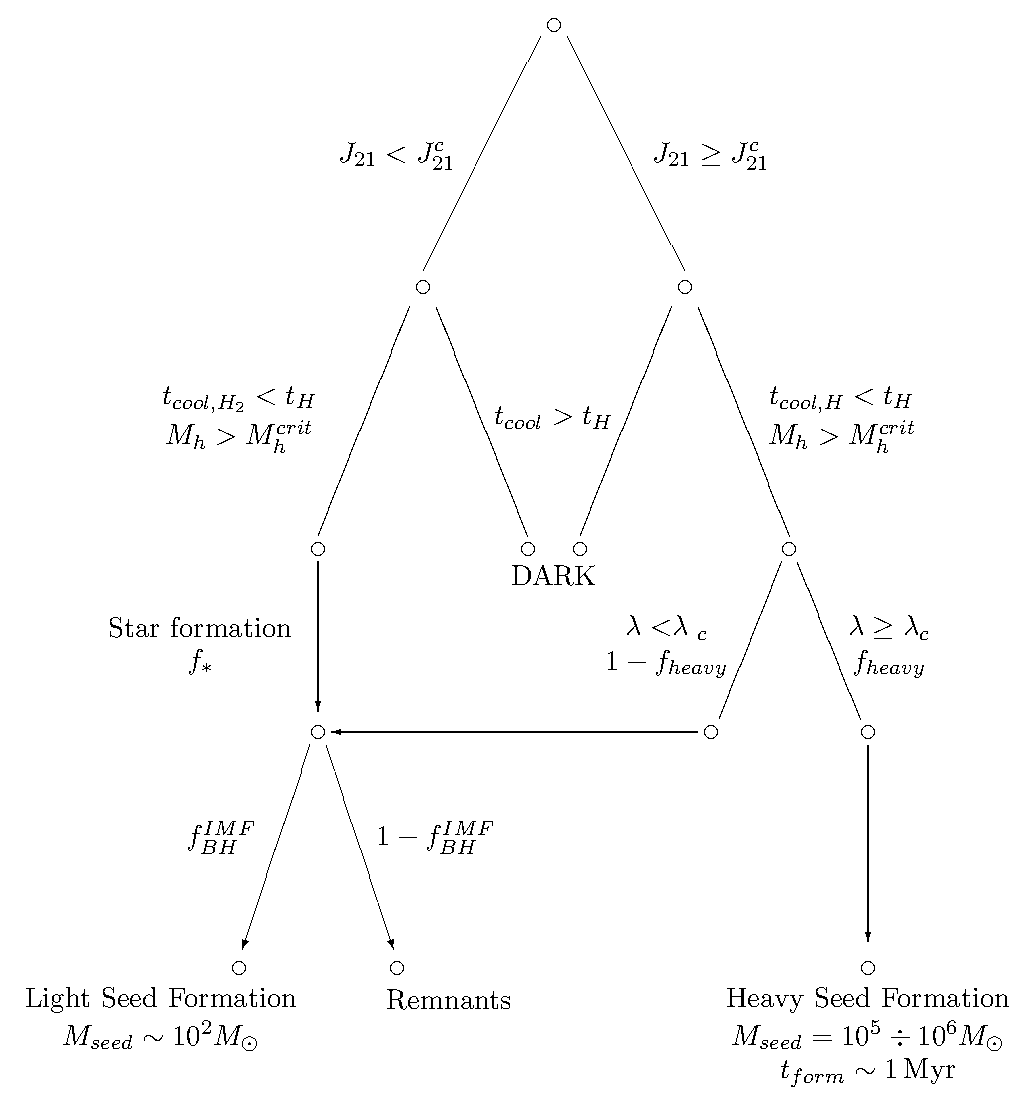
\includegraphics[scale=0.5]{Draw/seeding_scheme.pdf}
\end{center}
\caption{Schematic representation of the baryonic physics inside a dark matter halo}
\label{barscheme}
\end{figure}
Here $J_{21}$ is a parameter that quantifies the background radiation level in the $H_2$ photodissociation band, and $\lambda$ is a parameter that quantifies the angular spinning velocity of the halo. Without going too much in the details, what you should understand is that not all dark matter halos can host black hole seeds inside them, and the conditions for this to happen are pretty stringent and are strongly dependent on the physics of the gas contained in them. With the modern simulation tools that we have today we are able to compute the mass and number distribution of dark matter halos in the universe, which can be ultimately converted in a black hole mass and number distribution. That's basically how people were able to develop models that explain the presence of these supermassive black holes: with a suitable distribution of heavy black hole seeds which merge and accrete at the Eddington rate, it is actually possible to put a $10^9 M_\odot$ QuaSaR together. It is believed today that QuaSaRS are the glue that hold galaxies together, in the sense that each galaxy has its own QuaSaR at its center (for example the black hole that inhabits the center of the Milky Way, our galaxy, has a mass of $10^6 M_\odot$). This is also why these objects are also called Active Galactic Nuclei (AGN).   

\section{Observational prospects: gravitational waves}
All the things that we mentioned in the previous discussion might all seem very speculative, without solid observational evidence, and in a certain sense this is true. We have a strong evidence that AGNs are not fueled by stellar mechanisms, because of their non-thermal emission spectra (as shown in Figure \ref{quasarspecreal}). We also know that systems that accrete gas on a black hole at the Eddington rate typically exibit a non thermal spectrum like the one in Figure \ref{quasarspecreal}, and this is encouraging. How can we be really sure that these systems are black holes though? In the future in fact we hope to actually detect the black hole nature of AGNs with a new kind of telescope: these new telescopes are not sensible to electromagnetic waves (light), but to the gravitational waves that originate from black holes collisions. In the near future, we hope in fact to detect the gravitational bursts that originate from a collision of two dark matter halos (in particular of the black holes at their center). But what is a gravitational wave exactly? You might be familiar with sound waves: these are nothing more than perturbations in the air pressure that travel at the sound speed $c_s$ (that at room temperature is about 340\,m/s). In particular we can write down the pressure profile of a sound wave of frequency $\nu$ that travels in the $z$ direction for example
\begin{equation}
P(z,t)=P_0\sin{\left[2\pi\nu\left(\frac{z}{c_s}-t\right)\right]}
\end{equation}  
The range of human audible frequencies ranges from 20\,Hz to 20\,kHz. You are also familiar with electromagnetic waves, i.e. light: for these the quantity that oscillates is not the air pressure but the electric field instead. The propagation speed is the speed of light $c$; the electric field profile for an electromagnetic wave that travels in the $z$ direction can hence be written as 
\begin{equation}
\mathbf{E}(z,t) = \mathbf{E}_0\sin{\left[2\pi\nu\left(\frac{z}{c}-t\right)\right]}
\end{equation} 
Where the \textit{polarization vector} $\mathbf{E}_0$ is orthogonal to the direction of propagation (e.m. waves are \textit{transverse}) and can point in the $x$ or $y$ direction. Electromagnetic waves that can be seen by our naked eye have frequencies that span the \textit{visible spectrum} and range from 380 to 750\,THz (1\,THz = $10^3$\,GHz). When we talk about gravitational waves, we mean something really similar: in this case the quantity that oscillates is the spacetime metric $g_{\mu\nu}$ itself! At this point a typical profile of a gravitational wave looks familiar
\begin{equation}
g_{\mu\nu}(z,t) = g^0_{\mu\nu}\sin{\left[2\pi\nu\left(\frac{z}{c}-t\right)\right]}
\end{equation}
and the \textit{polarization tensor} $g^0_{\mu\nu}$ can be either of $+$ or $\times$ type. Take a look at the following links to see how a $+$ (\url{http://en.wikipedia.org/wiki/File:GravitationalWave_PlusPolarization.gif}) and $\times$ (\url{http://en.wikipedia.org/wiki/File:GravitationalWave_CrossPolarization.gif}) gravitational wave looks like (the figures show the spacetime deformations in the $(x,y)$ plane due to the passage of the wave). What is the typical frequency $\nu$ of the gravitational waves emitted in the collision of two black holes? We can give a simple estimate of this quantity if we know the mass scale $M$ of the system we are considering. Given a self gravitating system of density $\rho$, gravitational collapse will occur in a typical timescale $t_{grav}\sim\sqrt{1/G\rho}$. If we try to estimate the density for a black hole of mass $M$ we get $\rho\sim M/r_s^3 = c^6/8G^3M^2$, which translates in a wave frequency scale of $\nu_{grav} = 1/t_{grav} \sim c^3/GM$, or
\begin{equation}
\nu_{grav}\sim 10^5\,\mathrm{Hz}\frac{M_\odot}{M}
\end{equation}   
The gravitational frequency scale is inversely proportional to the mass of the system, and for a light $100M_\odot$ black hole collision it falls in the audible range! Of course the human ear is not sensible to gravitational waves, but we can always use a computer to convert a GW waveform in an audio signal (this is only because the frequency range is the right one!). Consider the following waveform in Figure \ref{waveform}, that is representative of a light black hole collision. 
\begin{figure}
\begin{center}
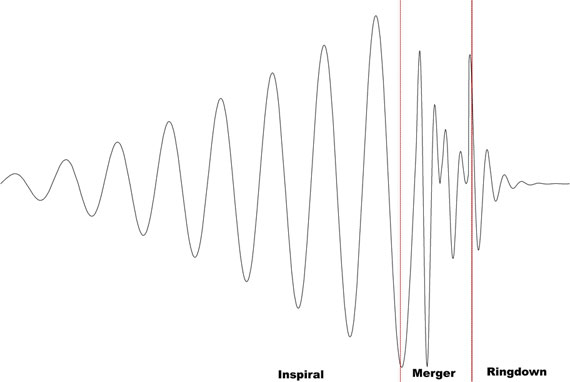
\includegraphics[scale=0.5]{Draw/GWwaveform.jpg}
\end{center}
\caption{Typical gravitational waveform generated in a black hole collision}
\label{waveform}
\end{figure}
This is how it sounds like, after digital signal processing and amplification: \url{http://www.youtube.com/watch?v=_9QpGy2QAkg}. Gravitational waves are a promising observational prospect for AGN physics in the future, unfortunately they are extremely weak and hard to detect. The energy per unit time carried by gravitational radiation generated in the collision of two black holes of masses $m_1$ and $m_2$ is given by
\begin{equation}
\dot{E}_{grav} = \frac{32G^4}{5c^5}\frac{m_1^2m_2^2(m_1+m_2)}{r^5}
\end{equation} 
which for a typical solar mass system with typical separation of a few $AU$ amounts to a few hundreds of W. This is comparable with the power emitted by the light bulb in your bedrooms. You can easily see how hard is the detection of gravitational radiation. An additional obstacle is that massive systems ($10^6\div 10^9 M_\odot$) generate gravitational waves of extremely low frequencies (fractions of Hz) and hence require extremely long observation times for detection. Nevertheless we still hope to use this tool to investigate the physics of black hole collisions, and gravitational wave astronomy is a rapidly growing and exciting field to go into.